\documentclass{article}   

\usepackage{geometry}
\usepackage{qtree}
\usepackage[square,numbers]{natbib}
% \usepackage{cite}  
\geometry{a4paper}

\usepackage[]{algorithm2e}
\usepackage{amsthm}
\newtheorem{theorem}{Theorem}[section]
\newtheorem{corollary}{Corollary}[theorem]
\newtheorem{example}{Example}
\newtheorem{lemma}[theorem]{Lemma}
\usepackage{rotating}
\usepackage[utf8]{inputenc}
\usepackage[T1]{fontenc}    % use 8-bit T1 fonts
\usepackage{lmodern}
\usepackage{hyperref}       % hyperlinks
\usepackage{lipsum}

%\usepackage[dvipsnames]{xcolor}
\usepackage{color, colortbl}

\definecolor{Gray}{gray}{0.9}
\definecolor{goldenpoppy}{rgb}{0.99, 0.76, 0.0}
\definecolor{goldenrod}{rgb}{0.85, 0.65, 0.13}

\usepackage[protrusion=true,expansion=true]{microtype}

\usepackage{amssymb}
\usepackage{amsfonts}
\usepackage{booktabs}
\usepackage{eqnarray,amsmath}
\usepackage[table]{xcolor}

\usepackage{listings}
\usepackage{dirtytalk}

\usepackage{rotating}
\usepackage{caption}

%% if you use PostScript figures in your article
%% use the graphics package for simple commands
\usepackage{graphics}


%% or use the graphicx package for more complicated commands
\usepackage{graphicx}


\usepackage{indentfirst}
\usepackage[utf8]{inputenc}
 \usepackage{subcaption}

 
\usepackage{xspace,color}
\usepackage{url}

\usepackage[export]{adjustbox}

\usepackage{listings}
\usepackage{xcolor}

\definecolor{codegreen}{rgb}{0,0.6,0}
\definecolor{codegray}{rgb}{0.5,0.5,0.5}
\definecolor{codepurple}{rgb}{0.58,0,0.82}
\definecolor{backcolour}{rgb}{0.95,0.95,0.92}

\lstdefinestyle{mystyle}{
    backgroundcolor=\color{backcolour},   
    commentstyle=\color{codegreen},
    keywordstyle=\color{magenta},
    numberstyle=\tiny\color{codegray},
    stringstyle=\color{codepurple},
    basicstyle=\ttfamily\footnotesize,
    breakatwhitespace=false,         
    breaklines=true,                 
    captionpos=b,                    
    keepspaces=true,                 
    numbers=left,                    
    numbersep=5pt,                  
    showspaces=false,                
    showstringspaces=false,
    showtabs=false,                  
    tabsize=2
}

\lstset{style=mystyle}

\newcommand{\ri}[1]{\lstinline{#1}}  %% Short for 'R inline'

\lstset{language=R}             % Set R to default language


%https://tex.stackexchange.com/questions/96825/nicely-formatted-where-statement-for-maths
 \newenvironment{where}{\noindent{}where\begin{itemize}}{\end{itemize}}
 \renewcommand*\descriptionlabel[1]{\hspace\leftmargin$#1$}
 
 %\newtheorem{theorem}{Theorem}[section]
%\newtheorem{corollary}{Corollary}[theorem]
%\newtheorem{lemma}[theorem]{Lemma}


\lstset{escapeinside={<@}{@>}}
% please place your own definitions here and don't use \def but
% \newcommand{}{}
%
% Insert the name of "your journal" with
% \journalname{myjournal}
%
\begin{document}

\title{%
  Practice 13: Law of large numbers. } %\\~\\
  %\Large }
\author{Mayra Cristina Berrones Reyes 6291}

\maketitle

\section{Introduction}

The Law of Large Numbers (LLN) is a theorem of probability theory, which describes the results of performing the same experiment a large number of times. In broad terms, this law states that the average of the results by a large number of trials should be close to the expected value, and as more trials are performed, this result should appear closer and closer \cite{dekking2005modern}.\\

Explained in a more mathematical approach, we have Theorem \ref{lln} for the LLN \cite{grinstead2012introduction}.\\

\begin{theorem}[\textbf{Law of Large Numbers}]
\label{lln}
Let  $X_1, X_2, ... , X_n $ be an independent trial process, with finite expected value $\mu = E(X_j)$ and finite variance $\sigma^2 = X(X_j)$. Let $S_n = X_1 + X_2 + ... + X_n.$ Then for any $\epsilon > 0,$
\[P \left( \Bigr \lvert \frac{S_n}{n} - \mu \Bigr \rvert \geq \epsilon \right) \rightarrow 0\]
as $n \rightarrow \infty.$ Equivalently,
\[P \left( \Bigr \lvert \frac{S_n}{n} - \mu \Bigr \rvert < \epsilon \right) \rightarrow 1\]
as $n \rightarrow \infty.$
\end{theorem}
\begin{flushright}
$\blacksquare$
\end{flushright}

\subsection{Example: Die roll}

To better understand the LLN we also have an example \ref{die} from the same book \cite{grinstead2012introduction}, replacing some things from the Theorem \ref{lln} we have, 

\begin{example}
\label{die}
Consider n rolls of a die. Let $X_j$ be the outcome of the jth roll. Then $S_n  = X_1 + X_2 + ... + X_n$ is the sum of the first n rolls. This is an independent trials process with $E(X_j) = 7/2$. Thus, by the Law of Large Numbers, for any $\epsilon > 0$
\[P \left( \Bigr \lvert \frac{S_n}{n} - \frac{7}{2} \Bigr \rvert \geq \epsilon \right) \rightarrow 0\]
as $n \rightarrow \infty.$ An equivalent way to state this is that, for any $\epsilon > 0$,
\[P \left( \Bigr \lvert \frac{S_n}{n} - \frac{7}{2} \Bigr \rvert < \epsilon \right) \rightarrow 1\]
as $n \rightarrow \infty.$
\end{example}
\begin{flushright}
$\blacksquare$
\end{flushright}

This example tells us that, according to the LLN if a large number of six sided fair dice are rolled, then the average of their values is likely to be close tho 3.5, with an increasing precision the more dice are rolled. Thanks to a tool from Wolfram we are able to visualize the different stages of this process in Figure \ref{fig1}.\\

\begin{figure}[]
\begin{subfigure}{.5\textwidth}
  \centering
  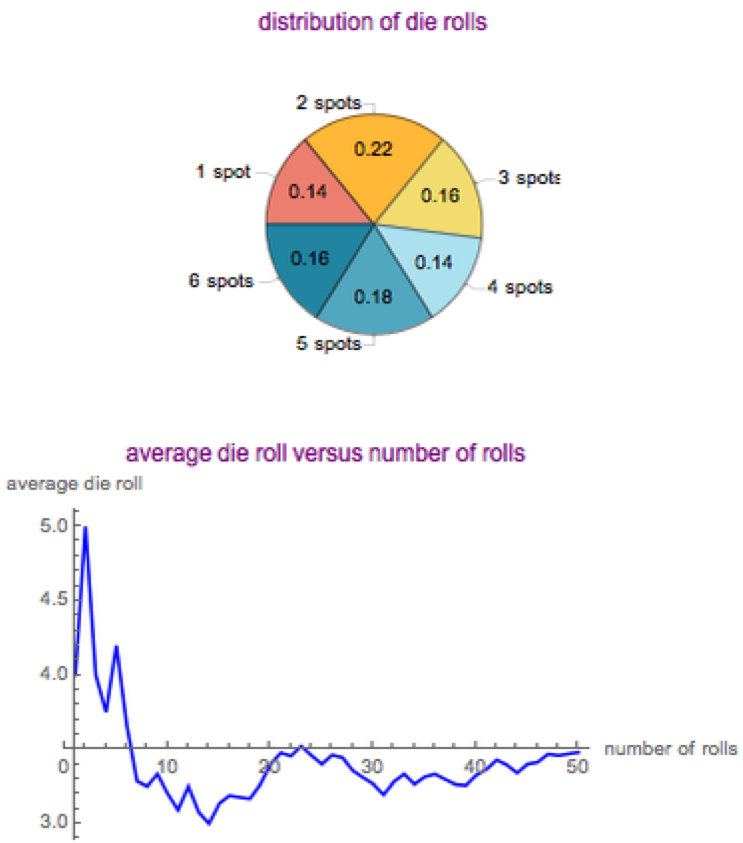
\includegraphics[width=.9\linewidth, left]{wolfram1.png}  
  \caption{50 rolls of the dice}
  \label{sb1-1}
\end{subfigure}\hspace{5mm}%
\begin{subfigure}{.5\textwidth}
  \centering
  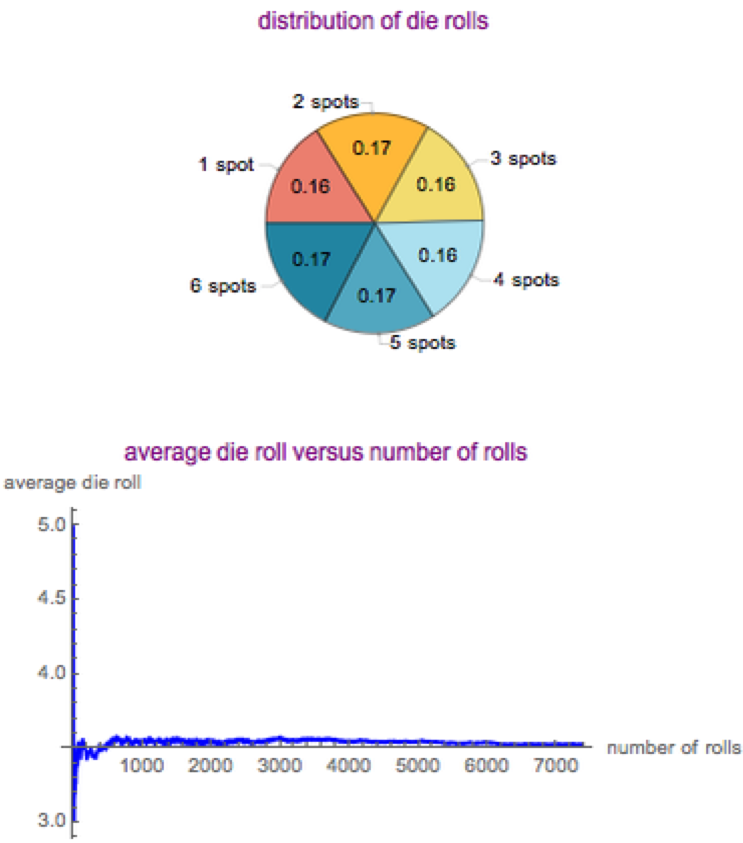
\includegraphics[width=.9\linewidth]{wolfram2.png}  
  \caption{7,500 rolls of the dice}
  \label{sb1-2}
\end{subfigure}\hspace{5mm}%
\newline
\begin{subfigure}{1\textwidth}
  \centering
  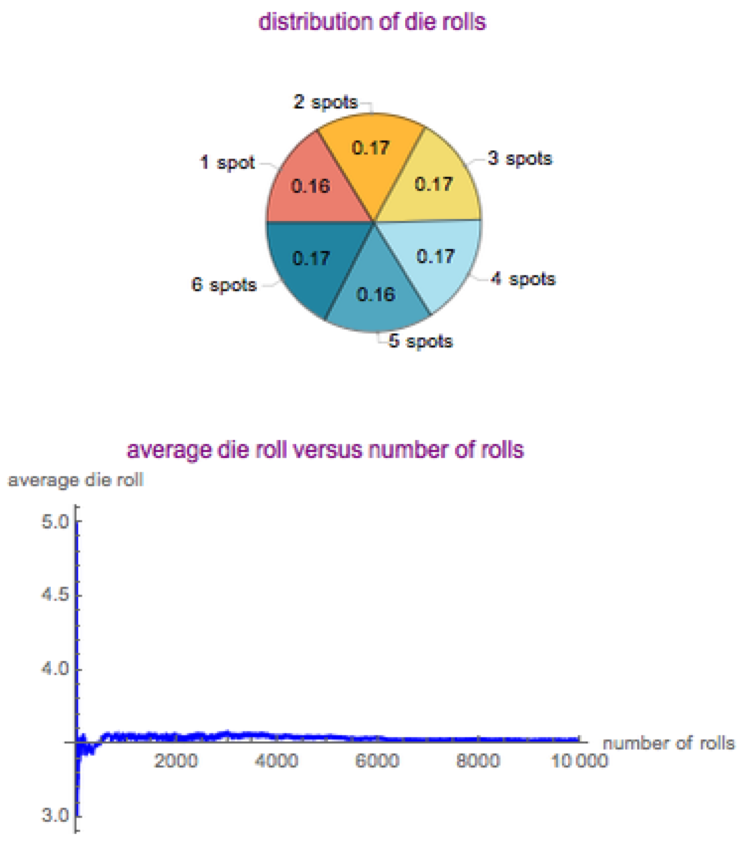
\includegraphics[width=.5\linewidth, center]{wolfram3.png}  
  \caption{10,000 rolls of the dice.}
  \label{sb1-3}
\end{subfigure}
	\caption{Different parameters for the dice experiment in the Wolfram page.}
\label{fig1}
\end{figure}

As we can see in Figure \ref{fig1} the mean is set to be 3.5, and as the iterations keep building, the line representing the average sum gets closer to converge to the mean line.\\

We can also develop a similar experiment in \texttt{R}, with simple functions such as \texttt{sample}. In this case, we take the average sum of two rolled dice. In Figure \ref{fig2} we represent with a lollipop plot the behavior of the different sizes of iterations of the experiment.\\

\begin{lstlisting}[language=R, caption=R extract of the code used to perform the dice experiment ]
two.dice <- function(){
  dice <- sample(1:6, size = 2, replace = TRUE)
  return(sum(dice))
}

two.dice()
replicate(n = 20, expr = two.dice())

sims <- replicate(100, two.dice())
table(sims)
df = as.data.frame(table(sims)/length(sims))
barplot(table(sims)/length(sims), xlab = 'Sum', ylab = 'Relative Frequency', main = '100 Rolls of 2 Fair Dice')

# Libraries
library(ggplot2)

# Create data
data <- data.frame(x=df$sims,y=df$Freq)

# Plot
png("Ej13_dice1.png", width = 1000, height = 1300, res = 300)
ggplot(data, aes(x=x, y=y)) +
  geom_segment( aes(x=x, xend=x, y=0, yend=y), color="grey") +
  geom_point( color="orange", size=4) +
  theme_light() +
  theme(panel.grid.major.x = element_blank(),
    panel.border = element_blank(),
    axis.ticks.x = element_blank()) +
  xlab("Sum") +
  ylab("Relative Frequency")
dev.off()

\end{lstlisting}

\begin{figure}[]
\begin{subfigure}{.5\textwidth}
  \centering
  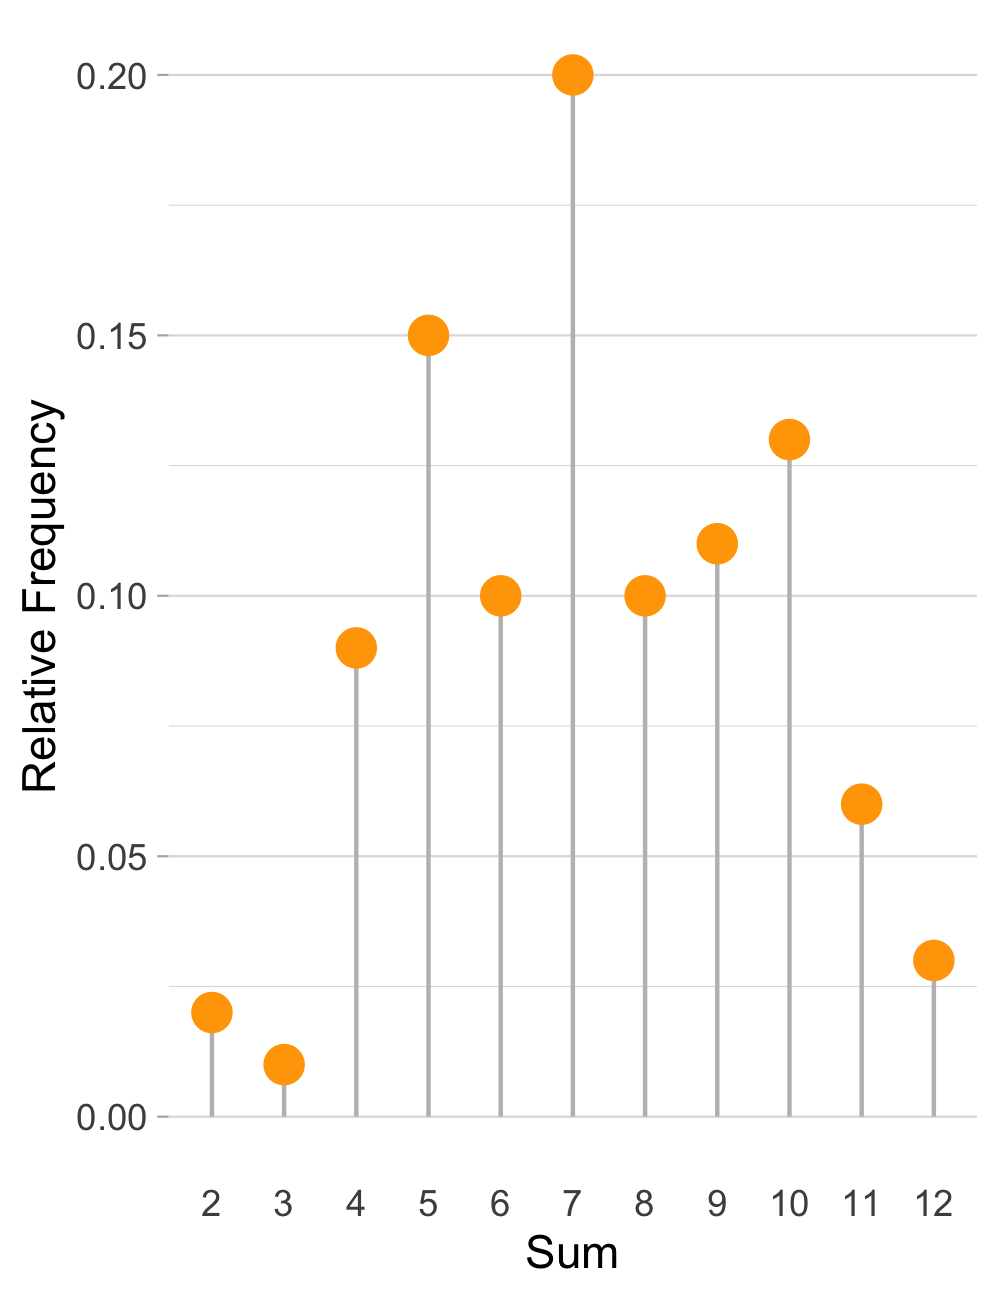
\includegraphics[width=.9\linewidth, left]{Ej13_dice1.png}  
  \caption{100 rolls of the dice}
  \label{sb2-1}
\end{subfigure}\hspace{5mm}%
\begin{subfigure}{.5\textwidth}
  \centering
  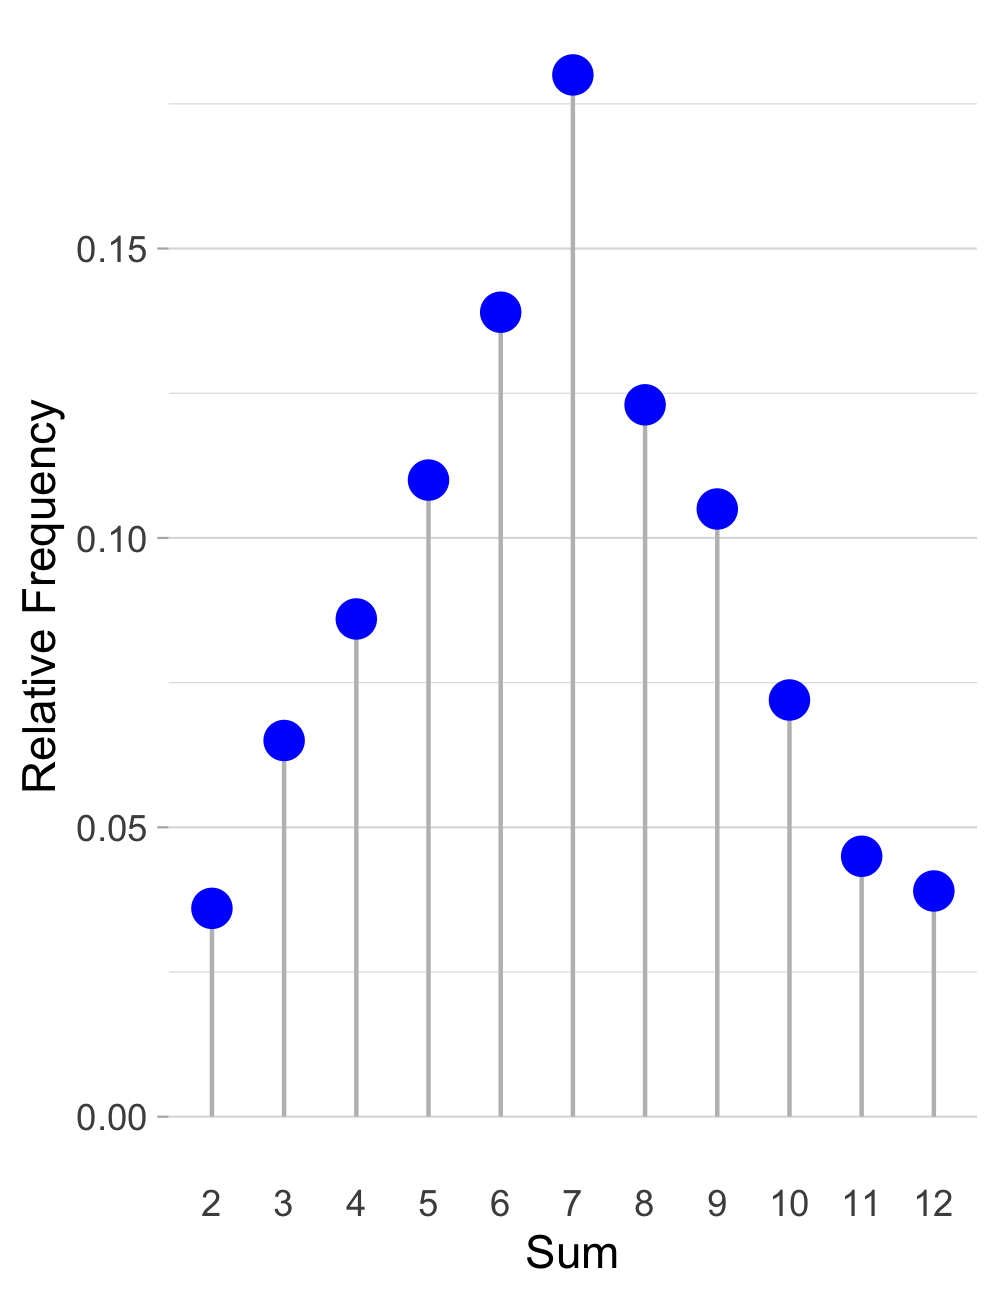
\includegraphics[width=.9\linewidth]{Ej13_dice2.png}  
  \caption{1,000 rolls of the dice}
  \label{sb2-2}
\end{subfigure}\hspace{5mm}%
\newline
\begin{subfigure}{1\textwidth}
  \centering
  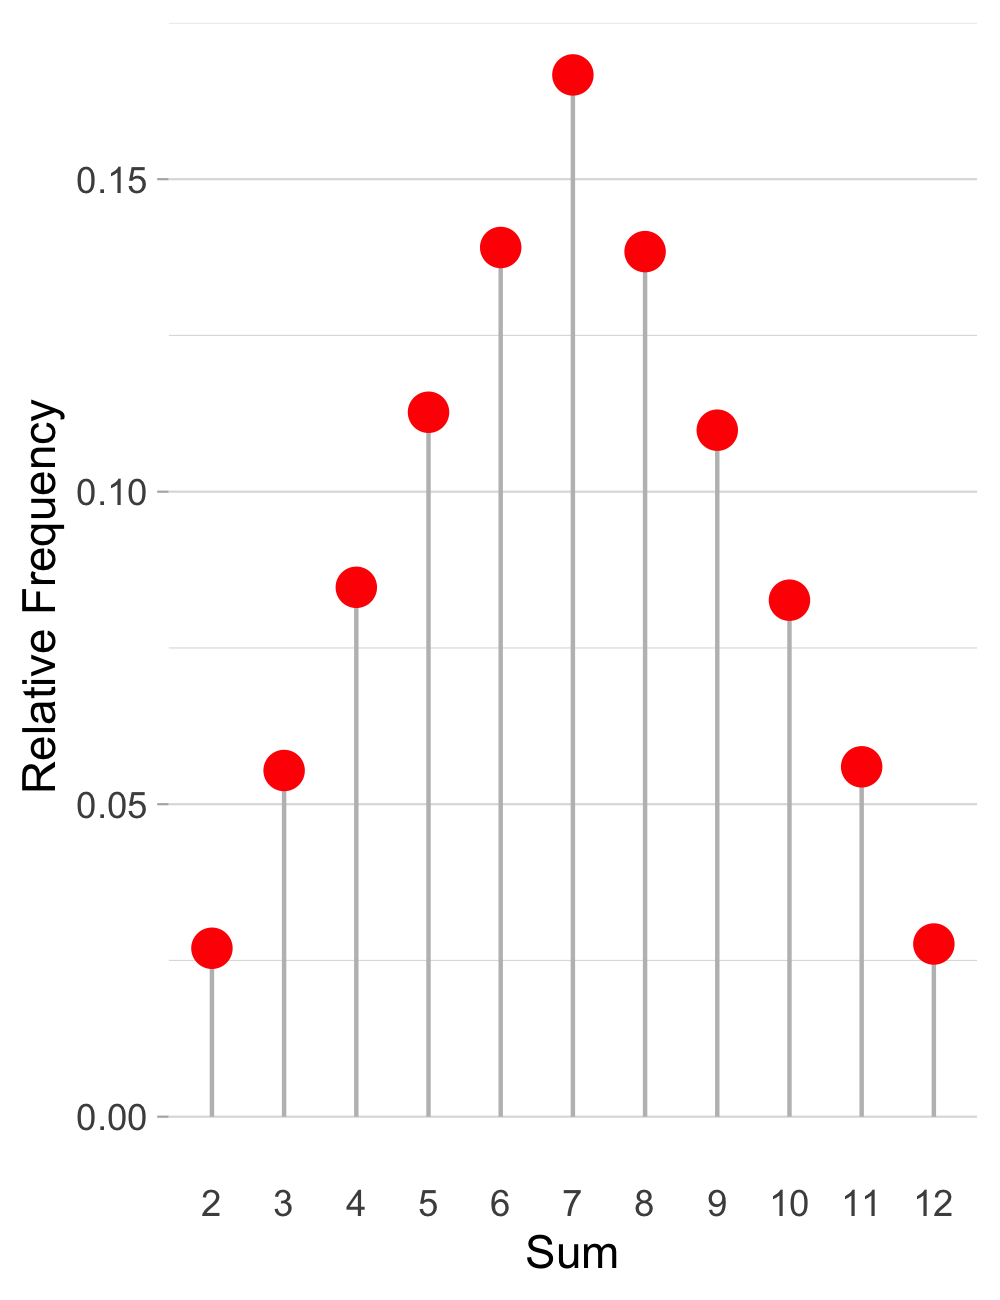
\includegraphics[width=.5\linewidth, center]{Ej13_dice3.png}  
  \caption{10,000 rolls of the dice.}
  \label{sb2-3}
\end{subfigure}
	\caption{Different parameters for the dice experiment performed in \texttt{R}.}
\label{fig2}
\end{figure}
\clearpage


\section{Applications of Law of Large Numbers in Machine Learning}

Now that the concept of the law of large number is presented, we searched for a topic related to the work of our thesis. In this case, there is a question that has always been present when working with Machine Learning tools such as Neural Networks (NN), and in this case is, how much data do I need to properly train my NN.\\

It all comes down to accuracy. When a experiment is performed, an accurate and precise result is desired. Accuracy of an experiment is defined as to whether or not the result of a measurement conforms to the correct value or expected value. Precision refers to the degree to which these values agree and can have a repeatable outcome if we performed the experiment again. The basic notion of this comes from the Law of Large Numbers (LLN), one of the basic principles of experimental physics and statistics. The law states that the average of an experiment performed many times converges to its true or expectation value.\\

In ML applications, this can translate as to training our NN with a defined set of data, and then testing this model with some more sets of data. The performance of the model we create depends upon the amount of data we use. When the data increases, we force the algorithm to fit the data, and with that, we minimize the error \cite{bot}. \\

In Figure \ref{fig3} we see the representation often used in articles to show the same behavior represented in the example of the dice \ref{fig1} we saw in the introduction, where we can see how the learning curve slowly flattens the more data we add to our model.\\

\begin{figure}[]
  \centering
  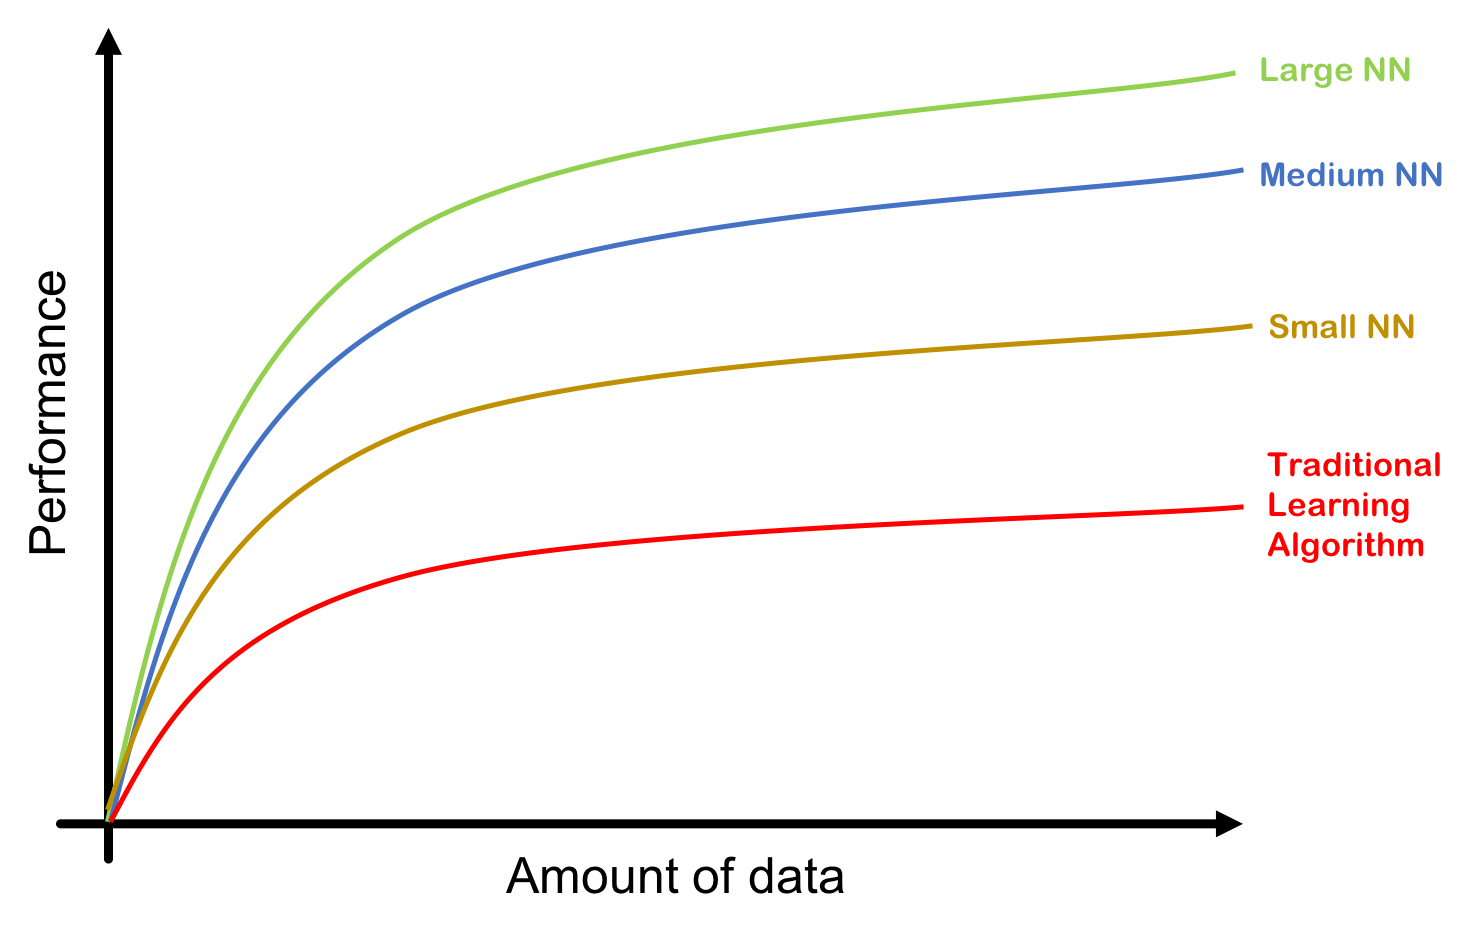
\includegraphics[width=.9\linewidth]{data1.png}  
	\caption{Representation of the learning curve with more amount of data.}
\label{fig3}
\end{figure}


Since our main goal is that our model gives us the best accuracy possible, we also have to consider the distribution of our data. Many cases have shown that the expected result of our test set will not match the accuracy performance of our training and developing sets if we use different distribution of data \cite{ng2017machine}. This also comes around to having a great amount of data to use for our model. Figure \ref{fig4} shows the \say{basic recipe} for machine learning. \\

\begin{figure}[]
  \centering
  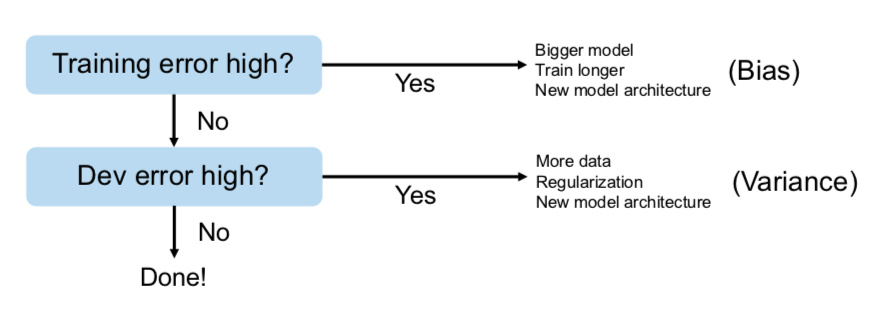
\includegraphics[width=.9\linewidth]{data2.png}  
	\caption{Basic recipe for machine learning \cite{ng2017machine}}
\label{fig4}
\end{figure}


As one Google Translate engineer put it, \say{when you go from 10,000 training examples to 10 billion training examples, it all starts to work. Data trumps everything}. \\

In our case, at the beginning of our Masters thesis \cite{tesis}, we started to develop toy CNN with the available data we had, which was not much. The maximum accuracy we could achieve for our image detection model, was of 65\% to 70\% in the test set. Later, when we were able to get more data sets, our accuracy improved to a 89\% accuracy.\\

As a final note, some of the things we learned along the way, is that is not always possible to have a large data set available to train our models, and in this case, there has been several application of transfer learning, that basically uses data form a different distribution (in our case, normal images, not medical ones) to pre train the wights of the NN, and improve the results of our training and testing. We are currenty looking for more examples of this in the medical field, since the ones we already found are lacking in accuracy performance.\\

\section{Conclusion}

The theory of Large Numbers applied in Machine Learning was something we heard of in a conference of the ENOAN in Zacatecas that we were able to attend. In this case, it was a really interesting topic for us, because in our mentioned masters thesis, we had a little idea when it came to one of the optimizers we used to perform our experiments in the architecture of the classification model for our CNN. \\

The SGD or Stochastic Gradient Decent optimizer, was one of the more robust algorithms used, since in all of the models we trained, it consistently kept upgrading the accuracy in the model, ending up in a steady 85\% to 95\%, and the difference in percentage from the training and tests sets where not so far apart. Even the optimizer we ended up using for the final experiment had some models in which the accuracy went bellow 40\%.\\

In the conference we mentioned, Dr. Hugo Estrada Esquivel with his lecture titled \say{Ciencia de datos en la era del internet de las cosas} \cite{enoan} commented about the experiments he had developed trying to stabilize the SGD optimizer. In his work, he found out, as we did, that the SGD optimizer is the most steady one, but also that it need significantly more time to converge in a optimal solution. Similar to the experiment in Figure \ref{fig1} it gets close to the desired output, but eventually swerves again.\\

We did not follow up with this investigation, because it was very costly (computational wise) to perform this type of experiments, but it would be very interesting to dig up again some information about it, to see if it has made some progress.\\

\bibliographystyle{plainnat}
\bibliography{tarea13}


 
\end{document}